\documentclass[12pt, twoside]{article}
% \documentclass[12pt, twoside]{article}
\usepackage[letterpaper, margin=1in, headsep=0.2in]{geometry}
\setlength{\headheight}{0.6in}
%\usepackage[english]{babel}
\usepackage[utf8]{inputenc}
\usepackage{microtype}
\usepackage{amsmath}
\usepackage{amssymb}
%\usepackage{amsfonts}
\usepackage[nomessages]{fp} %\FPeval{\var-name}{2*sin(pi/6)}
\usepackage{siunitx} %units in math. eg 20\milli\meter
\usepackage{yhmath} % for arcs, overparenth command
\usepackage{tikz} %graphics
\usetikzlibrary{quotes, angles, arrows, arrows.meta}
\usepackage{graphicx} %consider setting \graphicspath{{images/}}
\usepackage{parskip} %no paragraph indent
\usepackage{enumitem}
\usepackage{multicol}
\usepackage{venndiagram}

\usepackage{fancyhdr}
\pagestyle{fancy}
\fancyhf{}
\renewcommand{\headrulewidth}{0pt} % disable the underline of the header
\raggedbottom
\hfuzz=2mm %suppresses overfull box warnings

\usepackage{hyperref}
\usepackage{float}

\fancyhead[LE]{\thepage}
\fancyhead[RO]{\thepage \\ First and last name: \hspace{2.5cm} \,\\ Section: \hspace{2.5cm} \,}
\fancyhead[LO]{BECA/Huson/Geometry: Construction \\* 8 November 2024}

\begin{document}
\subsubsection*{2.12 Test: Applying triangle theorems}
\begin{enumerate}[itemsep=0.5cm]
\item Apply the Segment Addition postulate. Given $\overline{ABC}$ with $AB=11 \frac{1}{2}$ and $BC=6 \frac{1}{4}$. Find ${AC}$.\par  \vspace{0.5cm}
  \begin{tikzpicture}
    \draw [-, thick] (1,0)--(7,0);
    \draw [fill] (1,0) circle [radius=0.05] node[below]{$A$};
    \draw [fill] (5,0) circle [radius=0.05] node[below]{$B$};
    \draw [fill] (7,0) circle [radius=0.05] node[below]{$C$};
  \end{tikzpicture}  \vspace{3cm}

\item Apply the Angle Addition postulate. Write and equation to support your work.
\begin{multicols}{2}
  Given m$\angle ABD = 75^\circ$ and \\[0.25cm] m$\angle DBC = 30^\circ$. \\[0.5cm]
  Find $m \angle ABC$. \\
  \begin{tikzpicture}[scale=1.4]
    \draw[<->, thick]
      (3,0) coordinate (a) node[below left] {$C$}
      -- (0,0) coordinate (b) node[below left] {$B$}
      -- (2,1.5) coordinate (c) node[below right] {$D$}
      pic["$30^\circ$", <->, draw=black, angle eccentricity=1.5, angle radius=1cm]
      {angle=a--b--c};
      \draw[<-, thick]
      (-1,2) coordinate (d) node[right] {$A$}
      -- (0,0) coordinate (e)
      pic["$75^\circ$", <->, draw=black, angle eccentricity=1.25, angle radius=1cm]
      {angle=c--e--d};
  \end{tikzpicture}
\end{multicols} \vspace{2cm}

\item A triangle has two angles measuring $70^\circ$ and $60^\circ$ respectively. Find the measure of the third angle.
  \begin{flushright}
  \begin{tikzpicture}[scale=1]
    %\draw [->, thick] (0,0)--(5,5);
    \draw [-, thick] (0,0) node[xshift=0.6cm, yshift=0.4cm]{$70^\circ$}--
      (70:4) node[xshift=0.2cm, yshift=-0.7cm]{$60^\circ$}--
      (5,0) node[above, xshift=-0.7cm]{?}--cycle;
  \end{tikzpicture}
  \end{flushright} \vspace{2cm}


\newpage
\item Given  $\triangle EFG$ with $\overline{EF}$ extended to $A$. If $m\angle F=44^\circ$ and $m\angle G=92^\circ$, find $m\angle AEG$.
  \begin{center}
    \begin{tikzpicture}%[scale=0.7]
      \draw [thick](0,0)node[below]{$A$}--
        (2,0)node[below]{$E$}--
        (8,0)node[below]{$F$}--
        (4,3)node[above]{$G$} --(2,0);
    \end{tikzpicture}
  \end{center} \vspace{3cm}

\item Given $\triangle ABC$. $\overline{AC} \cong \overline{BC}$,  m$\angle A=75$. Find m$\angle C$.
  \begin{flushright}
  \begin{tikzpicture}[scale=0.7]
    \draw[thick](0,0)--(4,0)--(2,6)--(0,0);
    \draw[fill] (0,0) circle [radius=0.05] node[below]{$A$};
    \draw[fill] (4,0) circle [radius=0.05] node[below]{$B$};
    \draw[fill] (2,6) circle [radius=0.05] node[above right]{$C$};
    %\draw[color=blue] (0,0) ++(0.75,0) arc [start angle=0, end angle=70, radius=0.75];
    %\draw[color=blue] (4,0) ++(-0.22, 0.73) arc [start angle=110, end angle=180, radius=0.75];
    \draw[thick] (0.8,3.1)--(1.2,2.9); %tick mark
    \draw[thick] (2.8,2.9)--(3.2,3.1); %tick mark
    %\node [right] at (3.25,2.5){$x+7$};
    %\node [left] at (0.75,2.5){$2x+1$};
  \end{tikzpicture}
  \end{flushright}

\item The measures in degrees of the three angles of a triangle are $x$, $\frac{1}{2}x$, and $\frac{3}{2}x$. Find the measures of the triangle's angles.


\newpage
\item In $\triangle ABC$ shown below, $m\angle A=(5x+21)^\circ$, $m\angle B=(13x+4)^\circ$, and $m\angle C=(2x+15)^\circ$.\\[0.5cm] What is $m\angle A$?
\begin{flushright}
  \begin{tikzpicture}
    \draw [thick]
      (2,0)node[below]{$A$}--
      (9,0)node[below]{$C$}--
      (4,3)node[above]{$B$} --(2,0);
      \node at (3.3,0)[above]{$(5x+21)^\circ$};
      \node at (8.2,0)[above left]{$(2x+15)^\circ$};
      \node at (4.4,2.3)[below]{$(13x+4)^\circ$};
  \end{tikzpicture}
\end{flushright} \vspace{5cm}

\item In  $\triangle ABC$ shown below, side $\overline{AC}$ is extended to point $D$ with $m\angle DAB=(6x-16)^\circ$, $m\angle C=(x+4)^\circ$, and $m\angle B=(4x+3)^\circ$. \\[0.25cm]
Find $m\angle BAC$.
\begin{flushright}
    \begin{tikzpicture}[scale=0.9]
      \draw [thick](0,0)node[below]{$D$}--
        (1.8,0)node[below]{$A$}--
        (9,0)node[below]{$C$}--
        (4,3)node[above]{$B$} --(2,0);
        \node at (2.2,0)[above left]{$(6x-16)^\circ$};
        \node at (8.2,0)[above left]{$(x+4)^\circ$};
        \node at (4.4,2.4)[below]{$(4x+3)^\circ$};
    \end{tikzpicture}
  \end{flushright}


\newpage
\item A linear pair is formed by two angles, m$\angle RUT = 110^\circ$ and m$\angle SUT = 5x + 20$. \par \bigskip 
  Write an equation, then solve for $x$. \vspace{0.5cm}
    \begin{flushright}
      \begin{tikzpicture}[scale=1]
        \draw[<->, thick]
          (0:3) coordinate (a) node[below left] {$S$}
          -- (0,0) coordinate (b) node[below] {$U$}
          -- (65:3) coordinate (c) node[above right] {$T$}
          pic["$5x + 20$", <->, draw=black, angle eccentricity=1.5, angle radius=1.5cm]
          {angle=a--b--c};
          \draw[<-, thick]
          (180:3) coordinate (d) node[below] {$R$}
          -- (0,0) coordinate (e)
          pic["$110^\circ$", <->, draw=black, angle eccentricity=1.5, angle radius=1.5cm]
          {angle=c--e--d};
      \end{tikzpicture}
    \end{flushright} \vspace{3cm}

\item As shown below, two lines intersect making four angles: $\angle 1$, $\angle 2$, $\angle 3$, and $\angle 4$. Given that m$\angle 1= x+32$ and m$\angle 3=2x-8$, find m$\angle 1$.
  \begin{flushright}
    \begin{tikzpicture}[scale=1, rotate=0]
      \draw[<->, thick] (1,-1)--(8,1);
      \draw[<->, thick] (3,2)--(6,-2);
      \node at (2,.3){m$\angle 1= x+32$};
      \node at (6.5,-.3){m$\angle 3=2x-8$};
      \node at (5,1){2};
      \node at (4,-1){4};
    \end{tikzpicture}
    \end{flushright}


\newpage
\item Given two parallel lines and a transversal, with m$\angle 1 = 3x-10$ and m$\angle 8 = 2x + 32$. \\ Write an equation, then solve for $x$.
\begin{flushright}
  \begin{tikzpicture}[scale=1]
    \draw [<->, thick] (3,2)--(8,2);
    \draw [<->, thick] (2,0)--(7,0);
    \draw [<->, thick] (4,-1)--(5.5,3);
    \node at (4.5,0.3) [left]{$5$};
    \node at (4.5,0.3) [right]{$6$};
    \node at (4.3,-0.3) [left]{$7$};
    \node at (4.3,-0.3) [right]{$8$};
    \node at (5.2,2) [above left]{$1$};
    \node at (5.2,2) [above right]{$2$};
    \node at (5,2) [below left]{$3$};
    \node at (5,2) [below right]{$4$};
  \end{tikzpicture}
\end{flushright} \vspace{4cm}

\item Given m$\angle ABD = 4x-6$, m$\angle DBC = 5x+10$, and $m \angle ABC = 130^\circ$, as shown. \par \medskip
  Model the situation with an equation, then solve for $x$. Check your solution for full credit.
  \begin{flushright}
      \begin{tikzpicture}[scale=2, rotate=0]
        \draw[<->, thick]
          (-10:1.5) coordinate (a) node[below left] {$C$}
          -- (0,0) coordinate (b) node[below] {$B$}
          -- (70:2) coordinate (c) node[above right] {$D$}
          pic["$5x+10$", <->, draw=black, angle eccentricity=1.75, angle radius=1cm]
          {angle=a--b--c};
          \draw[<-, thick]
          (120:1.75) coordinate (d) node[below left] {$A$}
          -- (0,0) coordinate (e)
          pic["$4x-6$", <->, draw=black, angle eccentricity=1.5, angle radius=1cm]
          {angle=c--e--d};
      \end{tikzpicture}
    \end{flushright}


\newpage
\item Construct a perpendicular bisector of $\overline{PQ}$.  
  \vspace{3cm}
  \begin{center}
  \begin{tikzpicture}
    \draw [-, thick] (0,0)--(5,-3);
    \draw [fill] (0,0) circle [radius=0.05] node[below]{$P$};
    \draw [fill] (5,-3) circle [radius=0.05] node[below]{$Q$};
  \end{tikzpicture}
  \end{center} 
  \vspace{3cm}

\item Construct an angle bisector of the given angle.
  \vspace{2cm}
  \begin{center}
  \begin{tikzpicture}[rotate=-60]
    \draw [<->, thick] (-7,2)--(0,0)--(0.5,7);
    %\draw [fill] (0,0) circle [radius=0.05] node[below]{$A$};
  \end{tikzpicture}
  \end{center} \vspace{1cm}

\newpage
\item Reflect $\triangle ABC$ across the $y$-axis. Label the image $\triangle A'B'C'$.
\begin{center}
    \begin{tikzpicture}[scale=0.7]
    \draw [help lines] (-8,-6) grid (8,6);
    \draw [thick, <->] (-8.4,0) -- (8.4,0) node [right] {$x$};
    \draw [thick, <->] (0,-6.4)--(0,6.4) node [above] {$y$};  
    \draw [thick]
      (-1,4) node[above right] {$A$}--
      (-4,-1) node[below] {$B$}--
      (-1,-1) node[below right] {$C$}--cycle;  
  \end{tikzpicture}
\end{center}

\item Perform the translation $x \rightarrow x+4, y \rightarrow y+6$ on $\triangle DEF$. Label the image $\triangle D'E'F'$.
\begin{center}
    \begin{tikzpicture}[scale=.7]
    \draw [help lines] (-8,-6) grid (8,6);
    \draw [thick, <->] (-8.4,0) -- (8.4,0) node [right] {$x$};
    \draw [thick, <->] (0,-6.4)--(0,6.4) node [above] {$y$};  
    \draw [thick]
      (-2,-2) node[above right] {$D$}--
      (-5,-1) node[above left] {$E$}--
      (-5,-3) node[below left] {$F$}--cycle;  
  \end{tikzpicture}
\end{center}

\newpage
\item Rotate the triangle $180^\circ$ counterclockwise around the origin, $\triangle ABC \rightarrow \triangle A'B'C'$. Complete the table of the coordinates and plot and label the image on the grid. \vspace{0.5cm}
\begin{multicols}{2}
  $A(0,0) \rightarrow$ \\[0.7cm]
  $B(4,1) \rightarrow$ \\[0.7cm]
  $C(4,-1) \rightarrow$ \\[0.7cm]
    \begin{tikzpicture}[scale=.70]
    \draw [help lines] (-5,-5) grid (5,5);
    \draw [thick, <->] (-5.4,0) -- (5.4,0) node [right] {$x$};
    \draw [thick, <->] (0,-5.4)--(0,5.4) node [above] {$y$};  
    \draw [thick]
      (0,0) node[below left] {$A$}--
      (4,1) node[above right] {$B$}--
      (4,-1) node[below right] {$C$}--cycle;  
    \end{tikzpicture}
  \end{multicols}

\item A translation is applied to $\triangle ABC$ moving it up 3 and to the left 2.
\begin{enumerate}
  \item Write as coordinate pairs the vertices of the image, $\triangle A'B'C'$ \\[0.7cm]
  $A(5,2) \rightarrow$ \\[0.7cm]
  $B(7,-2) \rightarrow$ \\[0.7cm]
  $C(11,5) \rightarrow$ \\[0.2cm]
  \item Which triangle is larger, or are they the same size? Justify your answer.
\end{enumerate}



\end{enumerate}
\end{document}